\PassOptionsToPackage{dvipsnames,table}{xcolor}
\documentclass[10pt]{beamer}
\usepackage{Cours}

\begin{document}



\newcounter{numchap}
\setcounter{numchap}{1}
\newcounter{numframe}
\setcounter{numframe}{0}
\newcommand{\mframe}[1]{\frametitle{#1} \addtocounter{numframe}{1}}
\newcommand{\cnum}{\fbox{\textcolor{yellow}{\textbf{C\thenumchap}}}~}
\newcommand{\makess}[1]{\section{#1} \label{ss\thesection}}
\newcommand{\stitle}{\textcolor{yellow}{\textbf{\thesection. \nameref{ss\thesection}}}}

\definecolor{codebg}{gray}{0.90}
\definecolor{grispale}{gray}{0.95}
\definecolor{fluo}{rgb}{1,0.96,0.62}
\newminted[langageC]{c}{linenos=true,escapeinside=||,highlightcolor=fluo,tabsize=2,breaklines=true}
\newminted[codepython]{python}{linenos=true,escapeinside=||,highlightcolor=fluo,tabsize=2,breaklines=true}
% Inclusion complète (ou partiel en indiquant premiere et dernière ligne) d'un fichier C
\newcommand{\inputC}[3]{\begin{mdframed}[backgroundcolor=codebg] \inputminted[breaklines=true,fontsize=#3,linenos=true,highlightcolor=fluo,tabsize=2,highlightlines={#2}]{c}{#1} \end{mdframed}}
\newcommand{\inputpartC}[5]{\begin{mdframed}[backgroundcolor=codebg] \inputminted[breaklines=true,fontsize=#3,linenos=true,highlightcolor=fluo,tabsize=2,highlightlines={#2},firstline=#4,lastline=#5,firstnumber=1]{c}{#1} \end{mdframed}}
\newcommand{\inputpython}[3]{\begin{mdframed}[backgroundcolor=codebg] \inputminted[breaklines=true,fontsize=#3,linenos=true,highlightcolor=fluo,tabsize=2,highlightlines={#2}]{python}{#1} \end{mdframed}}
\newcommand{\inputpartOCaml}[5]{\begin{mdframed}[backgroundcolor=codebg] \inputminted[breaklines=true,fontsize=#3,linenos=true,highlightcolor=fluo,tabsize=2,highlightlines={#2},firstline=#4,lastline=#5,firstnumber=1]{OCaml}{#1} \end{mdframed}}
\BeforeBeginEnvironment{minted}{\begin{mdframed}[backgroundcolor=codebg]}
\AfterEndEnvironment{minted}{\end{mdframed}}
\newcommand{\kw}[1]{\textcolor{blue}{\tt #1}}

\newtcolorbox{rcadre}[4]{halign=center,colback={#1},colframe={#2},width={#3cm},height={#4cm},valign=center,boxrule=1pt,left=0pt,right=0pt}
\newtcolorbox{cadre}[4]{halign=center,colback={#1},colframe={#2},arc=0mm,width={#3cm},height={#4cm},valign=center,boxrule=1pt,left=0pt,right=0pt}
\newcommand{\myem}[1]{\colorbox{fluo}{#1}}
\mdfsetup{skipabove=1pt,skipbelow=-2pt}



% Noeud dans un cadre pour les arbres
\newcommand{\noeud}[2]{\Tr{\fbox{\textcolor{#1}{\tt #2}}}}

\newcommand{\htmlmode}{\lstset{language=html,numbers=left, tabsize=4, frame=single, breaklines=true, keywordstyle=\ttfamily, basicstyle=\small,
   numberstyle=\tiny\ttfamily, framexleftmargin=0mm, backgroundcolor=\color{grispale}, xleftmargin=12mm,showstringspaces=false}}
\newcommand{\pythonmode}{\lstset{
   language=python,
   linewidth=\linewidth,
   numbers=left,
   tabsize=4,
   frame=single,
   breaklines=true,
   keywordstyle=\ttfamily\color{blue},
   basicstyle=\small,
   numberstyle=\tiny\ttfamily,
   framexleftmargin=-2mm,
   numbersep=-0.5mm,
   backgroundcolor=\color{codebg},
   xleftmargin=-1mm, 
   showstringspaces=false,
   commentstyle=\color{gray},
   stringstyle=\color{OliveGreen},
   emph={turtle,Screen,Turtle},
   emphstyle=\color{RawSienna},
   morekeywords={setheading,goto,backward,forward,left,right,pendown,penup,pensize,color,speed,hideturtle,showturtle,forward}}
   }
   \newcommand{\Cmode}{\lstset{
      language=[ANSI]C,
      linewidth=\linewidth,
      numbers=left,
      tabsize=4,
      frame=single,
      breaklines=true,
      keywordstyle=\ttfamily\color{blue},
      basicstyle=\small,
      numberstyle=\tiny\ttfamily,
      framexleftmargin=0mm,
      numbersep=2mm,
      backgroundcolor=\color{codebg},
      xleftmargin=0mm, 
      showstringspaces=false,
      commentstyle=\color{gray},
      stringstyle=\color{OliveGreen},
      emphstyle=\color{RawSienna},
      escapechar=\|,
      morekeywords={}}
      }
\newcommand{\bashmode}{\lstset{language=bash,numbers=left, tabsize=2, frame=single, breaklines=true, basicstyle=\ttfamily,
   numberstyle=\tiny\ttfamily, framexleftmargin=0mm, backgroundcolor=\color{grispale}, xleftmargin=12mm, showstringspaces=false}}
\newcommand{\exomode}{\lstset{language=python,numbers=left, tabsize=2, frame=single, breaklines=true, basicstyle=\ttfamily,
   numberstyle=\tiny\ttfamily, framexleftmargin=13mm, xleftmargin=12mm, basicstyle=\small, showstringspaces=false}}
   
   
  
%tei pour placer les images
%tei{nom de l’image}{échelle de l’image}{sens}{texte a positionner}
%sens ="1" (droite) ou "2" (gauche)
\newlength{\ltxt}
\newcommand{\tei}[4]{
\setlength{\ltxt}{\linewidth}
\setbox0=\hbox{\includegraphics[scale=#2]{#1}}
\addtolength{\ltxt}{-\wd0}
\addtolength{\ltxt}{-10pt}
\ifthenelse{\equal{#3}{1}}{
\begin{minipage}{\wd0}
\includegraphics[scale=#2]{#1}
\end{minipage}
\hfill
\begin{minipage}{\ltxt}
#4
\end{minipage}
}{
\begin{minipage}{\ltxt}
#4
\end{minipage}
\hfill
\begin{minipage}{\wd0}
\includegraphics[scale=#2]{#1}
\end{minipage}
}
}

%Juxtaposition d'une image pspciture et de texte 
%#1: = code pstricks de l'image
%#2: largeur de l'image
%#3: hauteur de l'image
%#4: Texte à écrire
\newcommand{\ptp}[4]{
\setlength{\ltxt}{\linewidth}
\addtolength{\ltxt}{-#2 cm}
\addtolength{\ltxt}{-0.1 cm}
\begin{minipage}[b][#3 cm][t]{\ltxt}
#4
\end{minipage}\hfill
\begin{minipage}[b][#3 cm][c]{#2 cm}
#1
\end{minipage}\par
}



%Macros pour les graphiques
\psset{linewidth=0.5\pslinewidth,PointSymbol=x}
\setlength{\fboxrule}{0.5pt}
\newcounter{tempangle}

%Marque la longueur du segment d'extrémité  #1 et  #2 avec la valeur #3, #4 est la distance par rapport au segment (en %age de la valeur de celui ci) et #5 l'orientation du marquage : +90 ou -90
\newcommand{\afflong}[5]{
\pstRotation[RotAngle=#4,PointSymbol=none,PointName=none]{#1}{#2}[X] 
\pstHomO[PointSymbol=none,PointName=none,HomCoef=#5]{#1}{X}[Y]
\pstTranslation[PointSymbol=none,PointName=none]{#1}{#2}{Y}[Z]
 \ncline{|<->|,linewidth=0.25\pslinewidth}{Y}{Z} \ncput*[nrot=:U]{\footnotesize{#3}}
}
\newcommand{\afflongb}[3]{
\ncline{|<->|,linewidth=0}{#1}{#2} \naput*[nrot=:U]{\footnotesize{#3}}
}

%Construis le point #4 situé à #2 cm du point #1 avant un angle #3 par rapport à l'horizontale. #5 = liste de paramètre
\newcommand{\lsegment}[5]{\pstGeonode[PointSymbol=none,PointName=none](0,0){O'}(#2,0){I'} \pstTranslation[PointSymbol=none,PointName=none]{O'}{I'}{#1}[J'] \pstRotation[RotAngle=#3,PointSymbol=x,#5]{#1}{J'}[#4]}
\newcommand{\tsegment}[5]{\pstGeonode[PointSymbol=none,PointName=none](0,0){O'}(#2,0){I'} \pstTranslation[PointSymbol=none,PointName=none]{O'}{I'}{#1}[J'] \pstRotation[RotAngle=#3,PointSymbol=x,#5]{#1}{J'}[#4] \pstLineAB{#4}{#1}}

%Construis le point #4 situé à #3 cm du point #1 et faisant un angle de  90° avec la droite (#1,#2) #5 = liste de paramètre
\newcommand{\psegment}[5]{
\pstGeonode[PointSymbol=none,PointName=none](0,0){O'}(#3,0){I'}
 \pstTranslation[PointSymbol=none,PointName=none]{O'}{I'}{#1}[J']
 \pstInterLC[PointSymbol=none,PointName=none]{#1}{#2}{#1}{J'}{M1}{M2} \pstRotation[RotAngle=-90,PointSymbol=x,#5]{#1}{M1}[#4]
  }
  
%Construis le point #4 situé à #3 cm du point #1 et faisant un angle de  #5° avec la droite (#1,#2) #6 = liste de paramètre
\newcommand{\mlogo}[6]{
\pstGeonode[PointSymbol=none,PointName=none](0,0){O'}(#3,0){I'}
 \pstTranslation[PointSymbol=none,PointName=none]{O'}{I'}{#1}[J']
 \pstInterLC[PointSymbol=none,PointName=none]{#1}{#2}{#1}{J'}{M1}{M2} \pstRotation[RotAngle=#5,PointSymbol=x,#6]{#1}{M2}[#4]
  }

% Construis un triangle avec #1=liste des 3 sommets séparés par des virgules, #2=liste des 3 longueurs séparés par des virgules, #3 et #4 : paramètre d'affichage des 2e et 3 points et #5 : inclinaison par rapport à l'horizontale
%autre macro identique mais sans tracer les segments joignant les sommets
\noexpandarg
\newcommand{\Triangleccc}[5]{
\StrBefore{#1}{,}[\pointA]
\StrBetween[1,2]{#1}{,}{,}[\pointB]
\StrBehind[2]{#1}{,}[\pointC]
\StrBefore{#2}{,}[\coteA]
\StrBetween[1,2]{#2}{,}{,}[\coteB]
\StrBehind[2]{#2}{,}[\coteC]
\tsegment{\pointA}{\coteA}{#5}{\pointB}{#3} 
\lsegment{\pointA}{\coteB}{0}{Z1}{PointSymbol=none, PointName=none}
\lsegment{\pointB}{\coteC}{0}{Z2}{PointSymbol=none, PointName=none}
\pstInterCC{\pointA}{Z1}{\pointB}{Z2}{\pointC}{Z3} 
\pstLineAB{\pointA}{\pointC} \pstLineAB{\pointB}{\pointC}
\pstSymO[PointName=\pointC,#4]{C}{C}[C]
}
\noexpandarg
\newcommand{\TrianglecccP}[5]{
\StrBefore{#1}{,}[\pointA]
\StrBetween[1,2]{#1}{,}{,}[\pointB]
\StrBehind[2]{#1}{,}[\pointC]
\StrBefore{#2}{,}[\coteA]
\StrBetween[1,2]{#2}{,}{,}[\coteB]
\StrBehind[2]{#2}{,}[\coteC]
\tsegment{\pointA}{\coteA}{#5}{\pointB}{#3} 
\lsegment{\pointA}{\coteB}{0}{Z1}{PointSymbol=none, PointName=none}
\lsegment{\pointB}{\coteC}{0}{Z2}{PointSymbol=none, PointName=none}
\pstInterCC[PointNameB=none,PointSymbolB=none,#4]{\pointA}{Z1}{\pointB}{Z2}{\pointC}{Z1} 
}


% Construis un triangle avec #1=liste des 3 sommets séparés par des virgules, #2=liste formée de 2 longueurs et d'un angle séparés par des virgules, #3 et #4 : paramètre d'affichage des 2e et 3 points et #5 : inclinaison par rapport à l'horizontale
%autre macro identique mais sans tracer les segments joignant les sommets
\newcommand{\Trianglecca}[5]{
\StrBefore{#1}{,}[\pointA]
\StrBetween[1,2]{#1}{,}{,}[\pointB]
\StrBehind[2]{#1}{,}[\pointC]
\StrBefore{#2}{,}[\coteA]
\StrBetween[1,2]{#2}{,}{,}[\coteB]
\StrBehind[2]{#2}{,}[\angleA]
\tsegment{\pointA}{\coteA}{#5}{\pointB}{#3} 
\setcounter{tempangle}{#5}
\addtocounter{tempangle}{\angleA}
\tsegment{\pointA}{\coteB}{\thetempangle}{\pointC}{#4}
\pstLineAB{\pointB}{\pointC}
}
\newcommand{\TriangleccaP}[5]{
\StrBefore{#1}{,}[\pointA]
\StrBetween[1,2]{#1}{,}{,}[\pointB]
\StrBehind[2]{#1}{,}[\pointC]
\StrBefore{#2}{,}[\coteA]
\StrBetween[1,2]{#2}{,}{,}[\coteB]
\StrBehind[2]{#2}{,}[\angleA]
\lsegment{\pointA}{\coteA}{#5}{\pointB}{#3} 
\setcounter{tempangle}{#5}
\addtocounter{tempangle}{\angleA}
\lsegment{\pointA}{\coteB}{\thetempangle}{\pointC}{#4}
}

% Construis un triangle avec #1=liste des 3 sommets séparés par des virgules, #2=liste formée de 1 longueurs et de deux angle séparés par des virgules, #3 et #4 : paramètre d'affichage des 2e et 3 points et #5 : inclinaison par rapport à l'horizontale
%autre macro identique mais sans tracer les segments joignant les sommets
\newcommand{\Trianglecaa}[5]{
\StrBefore{#1}{,}[\pointA]
\StrBetween[1,2]{#1}{,}{,}[\pointB]
\StrBehind[2]{#1}{,}[\pointC]
\StrBefore{#2}{,}[\coteA]
\StrBetween[1,2]{#2}{,}{,}[\angleA]
\StrBehind[2]{#2}{,}[\angleB]
\tsegment{\pointA}{\coteA}{#5}{\pointB}{#3} 
\setcounter{tempangle}{#5}
\addtocounter{tempangle}{\angleA}
\lsegment{\pointA}{1}{\thetempangle}{Z1}{PointSymbol=none, PointName=none}
\setcounter{tempangle}{#5}
\addtocounter{tempangle}{180}
\addtocounter{tempangle}{-\angleB}
\lsegment{\pointB}{1}{\thetempangle}{Z2}{PointSymbol=none, PointName=none}
\pstInterLL[#4]{\pointA}{Z1}{\pointB}{Z2}{\pointC}
\pstLineAB{\pointA}{\pointC}
\pstLineAB{\pointB}{\pointC}
}
\newcommand{\TrianglecaaP}[5]{
\StrBefore{#1}{,}[\pointA]
\StrBetween[1,2]{#1}{,}{,}[\pointB]
\StrBehind[2]{#1}{,}[\pointC]
\StrBefore{#2}{,}[\coteA]
\StrBetween[1,2]{#2}{,}{,}[\angleA]
\StrBehind[2]{#2}{,}[\angleB]
\lsegment{\pointA}{\coteA}{#5}{\pointB}{#3} 
\setcounter{tempangle}{#5}
\addtocounter{tempangle}{\angleA}
\lsegment{\pointA}{1}{\thetempangle}{Z1}{PointSymbol=none, PointName=none}
\setcounter{tempangle}{#5}
\addtocounter{tempangle}{180}
\addtocounter{tempangle}{-\angleB}
\lsegment{\pointB}{1}{\thetempangle}{Z2}{PointSymbol=none, PointName=none}
\pstInterLL[#4]{\pointA}{Z1}{\pointB}{Z2}{\pointC}
}

%Construction d'un cercle de centre #1 et de rayon #2 (en cm)
\newcommand{\Cercle}[2]{
\lsegment{#1}{#2}{0}{Z1}{PointSymbol=none, PointName=none}
\pstCircleOA{#1}{Z1}
}

%construction d'un parallélogramme #1 = liste des sommets, #2 = liste contenant les longueurs de 2 côtés consécutifs et leurs angles;  #3, #4 et #5 : paramètre d'affichage des sommets #6 inclinaison par rapport à l'horizontale 
% meme macro sans le tracé des segements
\newcommand{\Para}[6]{
\StrBefore{#1}{,}[\pointA]
\StrBetween[1,2]{#1}{,}{,}[\pointB]
\StrBetween[2,3]{#1}{,}{,}[\pointC]
\StrBehind[3]{#1}{,}[\pointD]
\StrBefore{#2}{,}[\longueur]
\StrBetween[1,2]{#2}{,}{,}[\largeur]
\StrBehind[2]{#2}{,}[\angle]
\tsegment{\pointA}{\longueur}{#6}{\pointB}{#3} 
\setcounter{tempangle}{#6}
\addtocounter{tempangle}{\angle}
\tsegment{\pointA}{\largeur}{\thetempangle}{\pointD}{#5}
\pstMiddleAB[PointName=none,PointSymbol=none]{\pointB}{\pointD}{Z1}
\pstSymO[#4]{Z1}{\pointA}[\pointC]
\pstLineAB{\pointB}{\pointC}
\pstLineAB{\pointC}{\pointD}
}
\newcommand{\ParaP}[6]{
\StrBefore{#1}{,}[\pointA]
\StrBetween[1,2]{#1}{,}{,}[\pointB]
\StrBetween[2,3]{#1}{,}{,}[\pointC]
\StrBehind[3]{#1}{,}[\pointD]
\StrBefore{#2}{,}[\longueur]
\StrBetween[1,2]{#2}{,}{,}[\largeur]
\StrBehind[2]{#2}{,}[\angle]
\lsegment{\pointA}{\longueur}{#6}{\pointB}{#3} 
\setcounter{tempangle}{#6}
\addtocounter{tempangle}{\angle}
\lsegment{\pointA}{\largeur}{\thetempangle}{\pointD}{#5}
\pstMiddleAB[PointName=none,PointSymbol=none]{\pointB}{\pointD}{Z1}
\pstSymO[#4]{Z1}{\pointA}[\pointC]
}


%construction d'un cerf-volant #1 = liste des sommets, #2 = liste contenant les longueurs de 2 côtés consécutifs et leurs angles;  #3, #4 et #5 : paramètre d'affichage des sommets #6 inclinaison par rapport à l'horizontale 
% meme macro sans le tracé des segements
\newcommand{\CerfVolant}[6]{
\StrBefore{#1}{,}[\pointA]
\StrBetween[1,2]{#1}{,}{,}[\pointB]
\StrBetween[2,3]{#1}{,}{,}[\pointC]
\StrBehind[3]{#1}{,}[\pointD]
\StrBefore{#2}{,}[\longueur]
\StrBetween[1,2]{#2}{,}{,}[\largeur]
\StrBehind[2]{#2}{,}[\angle]
\tsegment{\pointA}{\longueur}{#6}{\pointB}{#3} 
\setcounter{tempangle}{#6}
\addtocounter{tempangle}{\angle}
\tsegment{\pointA}{\largeur}{\thetempangle}{\pointD}{#5}
\pstOrtSym[#4]{\pointB}{\pointD}{\pointA}[\pointC]
\pstLineAB{\pointB}{\pointC}
\pstLineAB{\pointC}{\pointD}
}

%construction d'un quadrilatère quelconque #1 = liste des sommets, #2 = liste contenant les longueurs des 4 côtés et l'angle entre 2 cotés consécutifs  #3, #4 et #5 : paramètre d'affichage des sommets #6 inclinaison par rapport à l'horizontale 
% meme macro sans le tracé des segements
\newcommand{\Quadri}[6]{
\StrBefore{#1}{,}[\pointA]
\StrBetween[1,2]{#1}{,}{,}[\pointB]
\StrBetween[2,3]{#1}{,}{,}[\pointC]
\StrBehind[3]{#1}{,}[\pointD]
\StrBefore{#2}{,}[\coteA]
\StrBetween[1,2]{#2}{,}{,}[\coteB]
\StrBetween[2,3]{#2}{,}{,}[\coteC]
\StrBetween[3,4]{#2}{,}{,}[\coteD]
\StrBehind[4]{#2}{,}[\angle]
\tsegment{\pointA}{\coteA}{#6}{\pointB}{#3} 
\setcounter{tempangle}{#6}
\addtocounter{tempangle}{\angle}
\tsegment{\pointA}{\coteD}{\thetempangle}{\pointD}{#5}
\lsegment{\pointB}{\coteB}{0}{Z1}{PointSymbol=none, PointName=none}
\lsegment{\pointD}{\coteC}{0}{Z2}{PointSymbol=none, PointName=none}
\pstInterCC[PointNameA=none,PointSymbolA=none,#4]{\pointB}{Z1}{\pointD}{Z2}{Z3}{\pointC} 
\pstLineAB{\pointB}{\pointC}
\pstLineAB{\pointC}{\pointD}
}


% Définition des colonnes centrées ou à droite pour tabularx
\newcolumntype{Y}{>{\centering\arraybackslash}X}
\newcolumntype{Z}{>{\flushright\arraybackslash}X}

%Les pointillés à remplir par les élèves
\newcommand{\po}[1]{\makebox[#1 cm]{\dotfill}}
\newcommand{\lpo}[1][3]{%
\multido{}{#1}{\makebox[\linewidth]{\dotfill}
}}

%Liste des pictogrammes utilisés sur la fiche d'exercice ou d'activités
\newcommand{\bombe}{\faBomb}
\newcommand{\livre}{\faBook}
\newcommand{\calculatrice}{\faCalculator}
\newcommand{\oral}{\faCommentO}
\newcommand{\surfeuille}{\faEdit}
\newcommand{\ordinateur}{\faLaptop}
\newcommand{\ordi}{\faDesktop}
\newcommand{\ciseaux}{\faScissors}
\newcommand{\danger}{\faExclamationTriangle}
\newcommand{\out}{\faSignOut}
\newcommand{\cadeau}{\faGift}
\newcommand{\flash}{\faBolt}
\newcommand{\lumiere}{\faLightbulb}
\newcommand{\compas}{\dsmathematical}
\newcommand{\calcullitteral}{\faTimesCircleO}
\newcommand{\raisonnement}{\faCogs}
\newcommand{\recherche}{\faSearch}
\newcommand{\rappel}{\faHistory}
\newcommand{\video}{\faFilm}
\newcommand{\capacite}{\faPuzzlePiece}
\newcommand{\aide}{\faLifeRing}
\newcommand{\loin}{\faExternalLink}
\newcommand{\groupe}{\faUsers}
\newcommand{\bac}{\faGraduationCap}
\newcommand{\histoire}{\faUniversity}
\newcommand{\coeur}{\faSave}
\newcommand{\python}{\faPython}
\newcommand{\os}{\faMicrochip}
\newcommand{\rd}{\faCubes}
\newcommand{\data}{\faColumns}
\newcommand{\web}{\faCode}
\newcommand{\prog}{\faFile}
\newcommand{\algo}{\faCogs}
\newcommand{\important}{\faExclamationCircle}
\newcommand{\maths}{\faTimesCircle}
% Traitement des données en tables
\newcommand{\tables}{\faColumns}
% Types construits
\newcommand{\construits}{\faCubes}
% Type et valeurs de base
\newcommand{\debase}{{\footnotesize \faCube}}
% Systèmes d'exploitation
\newcommand{\linux}{\faLinux}
\newcommand{\sd}{\faProjectDiagram}
\newcommand{\bd}{\faDatabase}

%Les ensembles de nombres
\renewcommand{\N}{\mathbb{N}}
\newcommand{\D}{\mathbb{D}}
\newcommand{\Z}{\mathbb{Z}}
\newcommand{\Q}{\mathbb{Q}}
\newcommand{\R}{\mathbb{R}}
\newcommand{\C}{\mathbb{C}}

%Ecriture des vecteurs
\newcommand{\vect}[1]{\vbox{\halign{##\cr 
  \tiny\rightarrowfill\cr\noalign{\nointerlineskip\vskip1pt} 
  $#1\mskip2mu$\cr}}}


%Compteur activités/exos et question et mise en forme titre et questions
\newcounter{numact}
\setcounter{numact}{1}
\newcounter{numseance}
\setcounter{numseance}{1}
\newcounter{numexo}
\setcounter{numexo}{0}
\newcounter{numprojet}
\setcounter{numprojet}{0}
\newcounter{numquestion}
\newcommand{\espace}[1]{\rule[-1ex]{0pt}{#1 cm}}
\newcommand{\Quest}[3]{
\addtocounter{numquestion}{1}
\begin{tabularx}{\textwidth}{X|m{1cm}|}
\cline{2-2}
\textbf{\sffamily{\alph{numquestion})}} #1 & \dots / #2 \\
\hline 
\multicolumn{2}{|l|}{\espace{#3}} \\
\hline
\end{tabularx}
}
\newcommand{\QuestR}[3]{
\addtocounter{numquestion}{1}
\begin{tabularx}{\textwidth}{X|m{1cm}|}
\cline{2-2}
\textbf{\sffamily{\alph{numquestion})}} #1 & \dots / #2 \\
\hline 
\multicolumn{2}{|l|}{\cor{#3}} \\
\hline
\end{tabularx}
}
\newcommand{\Pre}{{\sc nsi} 1\textsuperscript{e}}
\newcommand{\Term}{{\sc nsi} Terminale}
\newcommand{\Sec}{2\textsuperscript{e}}
\newcommand{\Exo}[2]{ \addtocounter{numexo}{1} \ding{113} \textbf{\sffamily{Exercice \thenumexo}} : \textit{#1} \hfill #2  \setcounter{numquestion}{0}}
\newcommand{\Projet}[1]{ \addtocounter{numprojet}{1} \ding{118} \textbf{\sffamily{Projet \thenumprojet}} : \textit{#1}}
\newcommand{\ExoD}[2]{ \addtocounter{numexo}{1} \ding{113} \textbf{\sffamily{Exercice \thenumexo}}  \textit{(#1 pts)} \hfill #2  \setcounter{numquestion}{0}}
\newcommand{\ExoB}[2]{ \addtocounter{numexo}{1} \ding{113} \textbf{\sffamily{Exercice \thenumexo}}  \textit{(Bonus de +#1 pts maximum)} \hfill #2  \setcounter{numquestion}{0}}
\newcommand{\Act}[2]{ \ding{113} \textbf{\sffamily{Activité \thenumact}} : \textit{#1} \hfill #2  \addtocounter{numact}{1} \setcounter{numquestion}{0}}
\newcommand{\Seance}{ \rule{1.5cm}{0.5pt}\raisebox{-3pt}{\framebox[4cm]{\textbf{\sffamily{Séance \thenumseance}}}}\hrulefill  \\
  \addtocounter{numseance}{1}}
\newcommand{\Acti}[2]{ {\footnotesize \ding{117}} \textbf{\sffamily{Activité \thenumact}} : \textit{#1} \hfill #2  \addtocounter{numact}{1} \setcounter{numquestion}{0}}
\newcommand{\titre}[1]{\begin{Large}\textbf{\ding{118}}\end{Large} \begin{large}\textbf{ #1}\end{large} \vspace{0.2cm}}
\newcommand{\QListe}[1][0]{
\ifthenelse{#1=0}
{\begin{enumerate}[partopsep=0pt,topsep=0pt,parsep=0pt,itemsep=0pt,label=\textbf{\sffamily{\arabic*.}},series=question]}
{\begin{enumerate}[resume*=question]}}
\newcommand{\SQListe}[1][0]{
\ifthenelse{#1=0}
{\begin{enumerate}[partopsep=0pt,topsep=0pt,parsep=0pt,itemsep=0pt,label=\textbf{\sffamily{\alph*)}},series=squestion]}
{\begin{enumerate}[resume*=squestion]}}
\newcommand{\SQListeL}[1][0]{
\ifthenelse{#1=0}
{\begin{enumerate*}[partopsep=0pt,topsep=0pt,parsep=0pt,itemsep=0pt,label=\textbf{\sffamily{\alph*)}},series=squestion]}
{\begin{enumerate*}[resume*=squestion]}}
\newcommand{\FinListe}{\end{enumerate}}
\newcommand{\FinListeL}{\end{enumerate*}}

%Mise en forme de la correction
\newcommand{\cor}[1]{\par \textcolor{OliveGreen}{#1}}
\newcommand{\br}[1]{\cor{\textbf{#1}}}
\newcommand{\tcor}[1]{\begin{tcolorbox}[width=0.92\textwidth,colback={white},colbacktitle=white,coltitle=OliveGreen,colframe=green!75!black,boxrule=0.2mm]   
\cor{#1}
\end{tcolorbox}
}
\newcommand{\rc}[1]{\textcolor{OliveGreen}{#1}}
\newcommand{\pmc}[1]{\textcolor{blue}{\tt #1}}
\newcommand{\tmc}[1]{\textcolor{RawSienna}{\tt #1}}


%Référence aux exercices par leur numéro
\newcommand{\refexo}[1]{
\refstepcounter{numexo}
\addtocounter{numexo}{-1}
\label{#1}}

%Séparation entre deux activités
\newcommand{\separateur}{\begin{center}
\rule{1.5cm}{0.5pt}\raisebox{-3pt}{\ding{117}}\rule{1.5cm}{0.5pt}  \vspace{0.2cm}
\end{center}}

%Entête et pied de page
\newcommand{\snt}[1]{\lhead{\textbf{SNT -- La photographie numérique} \rhead{\textit{Lycée Nord}}}}
\newcommand{\Activites}[2]{\lhead{\textbf{{\sc #1}}}
\rhead{Activités -- \textbf{#2}}
\cfoot{}}
\newcommand{\Exos}[2]{\lhead{\textbf{Fiche d'exercices: {\sc #1}}}
\rhead{Niveau: \textbf{#2}}
\cfoot{}}
\newcommand{\Devoir}[2]{\lhead{\textbf{Devoir de mathématiques : {\sc #1}}}
\rhead{\textbf{#2}} \setlength{\fboxsep}{8pt}
\begin{center}
%Titre de la fiche
\fbox{\parbox[b][1cm][t]{0.3\textwidth}{Nom : \hfill \po{3} \par \vfill Prénom : \hfill \po{3}} } \hfill 
\fbox{\parbox[b][1cm][t]{0.6\textwidth}{Note : \po{1} / 20} }
\end{center} \cfoot{}}

%Devoir programmation en NSI (pas à rendre sur papier)
\newcommand{\PNSI}[2]{\lhead{\textbf{Devoir de {\sc nsi} : \textsf{ #1}}}
\rhead{\textbf{#2}} \setlength{\fboxsep}{8pt}
\begin{tcolorbox}[title=\textcolor{black}{\danger\; A lire attentivement},colbacktitle=lightgray]
{\begin{enumerate}
\item Rendre tous vous programmes en les envoyant par mail à l'adresse {\tt fnativel2@ac-reunion.fr}, en précisant bien dans le sujet vos noms et prénoms
\item Un programme qui fonctionne mal ou pas du tout peut rapporter des points
\item Les bonnes pratiques de programmation (clarté et lisiblité du code) rapportent des points
\end{enumerate}
}
\end{tcolorbox}
 \cfoot{}}


%Devoir de NSI
\newcommand{\DNSI}[2]{\lhead{\textbf{Devoir de {\sc nsi} : \textsf{ #1}}}
\rhead{\textbf{#2}} \setlength{\fboxsep}{8pt}
\begin{center}
%Titre de la fiche
\fbox{\parbox[b][1cm][t]{0.3\textwidth}{Nom : \hfill \po{3} \par \vfill Prénom : \hfill \po{3}} } \hfill 
\fbox{\parbox[b][1cm][t]{0.6\textwidth}{Note : \po{1} / 10} }
\end{center} \cfoot{}}

\newcommand{\DevoirNSI}[2]{\lhead{\textbf{Devoir de {\sc nsi} : {\sc #1}}}
\rhead{\textbf{#2}} \setlength{\fboxsep}{8pt}
\cfoot{}}

%La définition de la commande QCM pour auto-multiple-choice
%En premier argument le sujet du qcm, deuxième argument : la classe, 3e : la durée prévue et #4 : présence ou non de questions avec plusieurs bonnes réponses
\newcommand{\QCM}[4]{
{\large \textbf{\ding{52} QCM : #1}} -- Durée : \textbf{#3 min} \hfill {\large Note : \dots/10} 
\hrule \vspace{0.1cm}\namefield{}
Nom :  \textbf{\textbf{\nom{}}} \qquad \qquad Prénom :  \textbf{\prenom{}}  \hfill Classe: \textbf{#2}
\vspace{0.2cm}
\hrule  
\begin{itemize}[itemsep=0pt]
\item[-] \textit{Une bonne réponse vaut un point, une absence de réponse n'enlève pas de point. }
\item[\danger] \textit{Une mauvaise réponse enlève un point.}
\ifthenelse{#4=1}{\item[-] \textit{Les questions marquées du symbole \multiSymbole{} peuvent avoir plusieurs bonnes réponses possibles.}}{}
\end{itemize}
}
\newcommand{\DevoirC}[2]{
\renewcommand{\footrulewidth}{0.5pt}
\lhead{\textbf{Devoir de mathématiques : {\sc #1}}}
\rhead{\textbf{#2}} \setlength{\fboxsep}{8pt}
\fbox{\parbox[b][0.4cm][t]{0.955\textwidth}{Nom : \po{5} \hfill Prénom : \po{5} \hfill Classe: \textbf{1}\textsuperscript{$\dots$}} } 
\rfoot{\thepage} \cfoot{} \lfoot{Lycée Nord}}
\newcommand{\DevoirInfo}[2]{\lhead{\textbf{Evaluation : {\sc #1}}}
\rhead{\textbf{#2}} \setlength{\fboxsep}{8pt}
 \cfoot{}}
\newcommand{\DM}[2]{\lhead{\textbf{Devoir maison à rendre le #1}} \rhead{\textbf{#2}}}

%Macros permettant l'affichage des touches de la calculatrice
%Touches classiques : #1 = 0 fond blanc pour les nombres et #1= 1gris pour les opérations et entrer, second paramètre=contenu
%Si #2=1 touche arrondi avec fond gris
\newcommand{\TCalc}[2]{
\setlength{\fboxsep}{0.1pt}
\ifthenelse{#1=0}
{\psframebox[fillstyle=solid, fillcolor=white]{\parbox[c][0.25cm][c]{0.6cm}{\centering #2}}}
{\ifthenelse{#1=1}
{\psframebox[fillstyle=solid, fillcolor=lightgray]{\parbox[c][0.25cm][c]{0.6cm}{\centering #2}}}
{\psframebox[framearc=.5,fillstyle=solid, fillcolor=white]{\parbox[c][0.25cm][c]{0.6cm}{\centering #2}}}
}}
\newcommand{\Talpha}{\psdblframebox[fillstyle=solid, fillcolor=white]{\hspace{-0.05cm}\parbox[c][0.25cm][c]{0.65cm}{\centering \scriptsize{alpha}}} \;}
\newcommand{\Tsec}{\psdblframebox[fillstyle=solid, fillcolor=white]{\parbox[c][0.25cm][c]{0.6cm}{\centering \scriptsize 2nde}} \;}
\newcommand{\Tfx}{\psdblframebox[fillstyle=solid, fillcolor=white]{\parbox[c][0.25cm][c]{0.6cm}{\centering \scriptsize $f(x)$}} \;}
\newcommand{\Tvar}{\psframebox[framearc=.5,fillstyle=solid, fillcolor=white]{\hspace{-0.22cm} \parbox[c][0.25cm][c]{0.82cm}{$\scriptscriptstyle{X,T,\theta,n}$}}}
\newcommand{\Tgraphe}{\psdblframebox[fillstyle=solid, fillcolor=white]{\hspace{-0.08cm}\parbox[c][0.25cm][c]{0.68cm}{\centering \tiny{graphe}}} \;}
\newcommand{\Tfen}{\psdblframebox[fillstyle=solid, fillcolor=white]{\hspace{-0.08cm}\parbox[c][0.25cm][c]{0.68cm}{\centering \tiny{fenêtre}}} \;}
\newcommand{\Ttrace}{\psdblframebox[fillstyle=solid, fillcolor=white]{\parbox[c][0.25cm][c]{0.6cm}{\centering \scriptsize{trace}}} \;}

% Macroi pour l'affichage  d'un entier n dans  une base b
\newcommand{\base}[2]{ \overline{#1}^{#2}}
% Intervalle d'entiers
\newcommand{\intN}[2]{\llbracket #1; #2 \rrbracket}}

% Numéro et titre de chapitre
\setcounter{numchap}{17}
\newcommand{\Ctitle}{\cnum {Graphes}}
\newcommand{\SPATH}{/home/fenarius/Travail/Cours/cpge-info/docs/mp2i/files/C\thenumchap/}
\newcommand{\ar}[1]{\{#1\}}

\makess{Exemples introductifs}
\begin{frame}[fragile]{\Ctitle}{\stitle}
	\begin{block}{Les sept ponts de Konigsberg}
		\begin{center}
			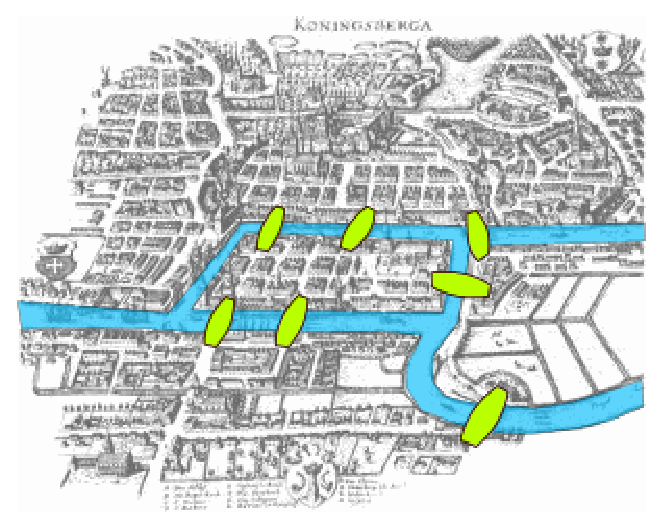
\includegraphics[width=160px]{konigsberg_bridges.eps}\\
			{\footnotesize credit : Wikipedia}
		\end{center}
		Est-il possible de trouver un chemin qui passe une seule fois par chaque pont ?
	\end{block}
\end{frame}

\begin{frame}[fragile]{\Ctitle}{\stitle}
	\begin{block}{Le problème des quatre couleurs}
		\begin{center}
			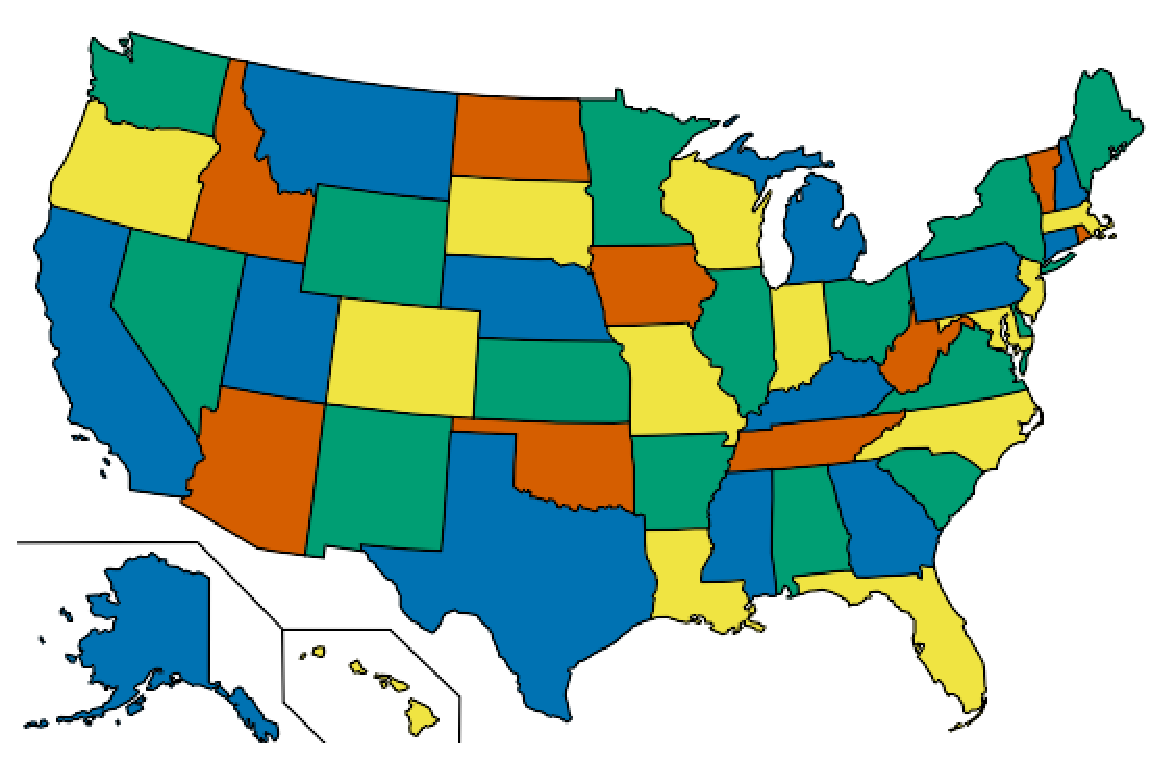
\includegraphics[width=160px]{US4.eps}\\
			{\footnotesize credit : Wikipedia}
		\end{center}
		Peut-on colorier n'importe quelle carte en utilisant seulement 4 couleurs ? (sans que deux pays limitrophes aient la même couleur)
	\end{block}
\end{frame}

\begin{frame}[fragile]{\Ctitle}{\stitle}
	\begin{block}{Le problème du voyageur de commerce}
		\begin{center}
			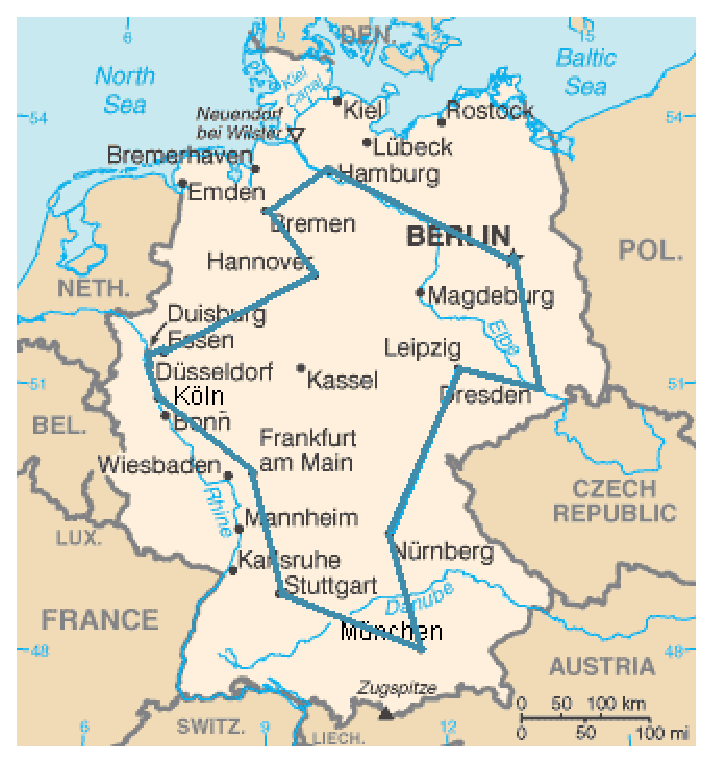
\includegraphics[height=130px]{TSP_Deutschland.eps}\\
			{\footnotesize credit : Wikipedia}
		\end{center}
		Trouver le chemin le plus court possible qui passe par toutes les villes une seule fois et revient à son point de départ.
	\end{block}
\end{frame}


\begin{frame}[fragile]{\Ctitle}{\stitle}
	\begin{block}{Le jeu de Juniper Green}
		\begin{center}
			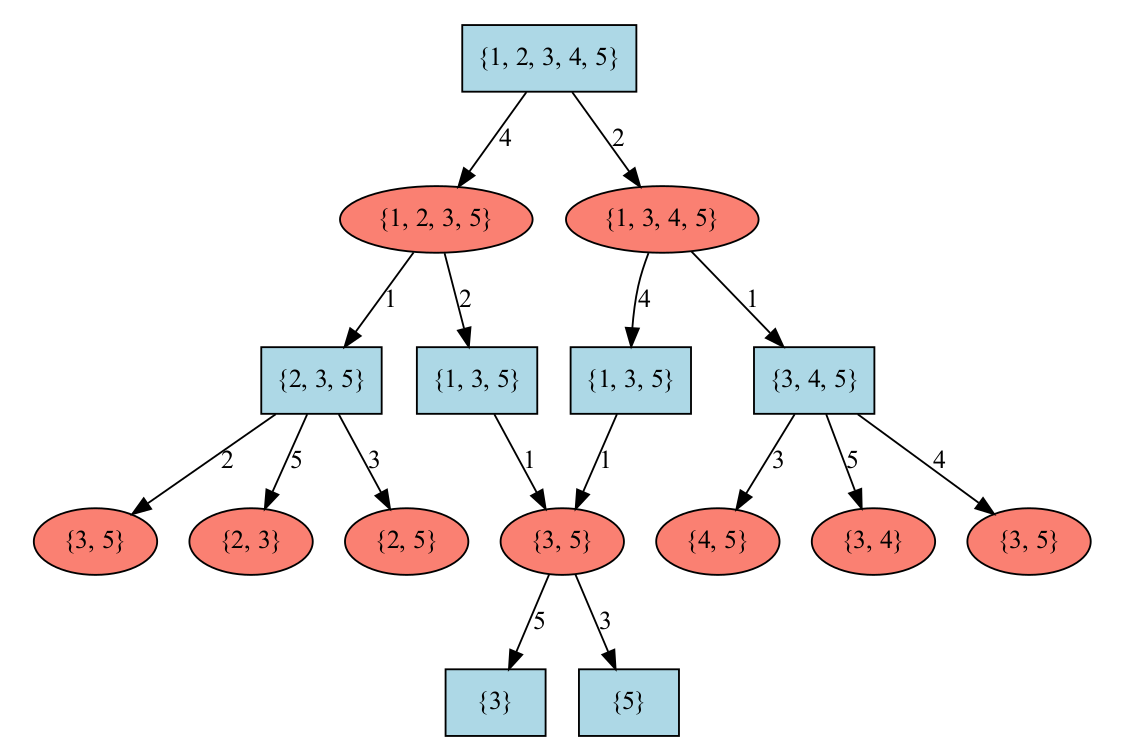
\includegraphics[width=200px]{juniper5.eps}\\
		\end{center}
		Existe-il une stratégie gagnante au jeu de Juniper Green ?
	\end{block}
\end{frame}

\begin{frame}[fragile]{\Ctitle}{\stitle}
	\begin{block}{Théorie des graphes}
		Ces problèmes se modélisent et se résolvent à l'aide de la \textcolor{blue}{théorie des graphes}, un domaine central de l'informatique ayant des applications variées :
		\begin{itemize}
			\item<1-> {\sc gps} : recherches de chemins,
			\item<2-> planification de tâches,
			\item<3-> réseaux : informatique, sociaux,
			\item<4-> énergie, transport, \dots
		\end{itemize}
		\onslide<5->{La taille des graphes en jeu impose la recherche d'algorithmes efficaces :}
		\onslide<6->{
			\begin{center}
				\begin{tabularx}{0.7\linewidth}{XXX}
					\textcolor{blue}{Graphe}                 & \textcolor{blue}{Sommets}                          & \textcolor{blue}{Arcs}                          \\
					\hline
					\leavevmode{\onslide<7->{Facebook}}      & \leavevmode{\onslide<7->{$\simeq 7,2\times 10^8$}} & \leavevmode{\onslide<7->{$\simeq 7\times10^9$}} \\
					\leavevmode{\onslide<8->{OpenStreetMap}} & \leavevmode{\onslide<8->{$\simeq 9\times 10^9$}}   & \leavevmode{\onslide<8->{$\simeq 10^9$}}        \\
					\leavevmode{\onslide<9->{Jeu d'échecs}}  & \leavevmode{\onslide<9->{$\simeq  10^{47}$}}       & \leavevmode{\onslide<9->{?}}                    \\
				\end{tabularx}
			\end{center}}
	\end{block}
\end{frame}

\makess{Définition et vocabulaire des graphes}
\begin{frame}[fragile]{\Ctitle}{\stitle}
	\begin{alertblock}{Définition}
		\onslide<1->{Un \textcolor{red}{graphe non-orienté} est la donnée :}
		\begin{itemize}
			\item<2->{D'un ensemble de \textcolor{blue}{sommets} (ou \textcolor{blue}{n\oe{}uds}) $S$ fini (\textcolor{gray}{V pour \textit{vertice} en anglais.}).}
			\item<3->{D'un ensemble de paires de sommets $A$ appelés \textcolor{blue}{arêtes} (\textcolor{gray}{E pour \textit{edges} en anglais}).}
		\end{itemize}
	\end{alertblock}
	\onslide<4->{\begin{block}{Remarques}
			\begin{itemize}
				\item<5-> Une arête est donc une paire $\{x, y \}$, avec $x \in S$, $y \in S$ et $x \neq y$.
				\item<6-> Puisque $\{x, y \} = \{ y, x \}$, l'ordre n'a pas d'importance.
				\item<7-> On notera $ x \relbar y$ ou plus simplement $xy$ l'arête $\{x, y \}$.
			\end{itemize}
		\end{block}}
\end{frame}

% Premiers exemples
\begin{frame}[fragile]{\Ctitle}{\stitle}
	\begin{exampleblock}{Exemple}
		\begin{pspicture}(0,2)(5,4)
			\rput(0.2,2.8){\Circlenode{S1}{$a$}}
			\rput(2,3){\Circlenode{S2}{$b$}}
			\rput(4,2){\Circlenode{S3}{$c$}}
			\rput(8,3){\Circlenode{S4}{$d$}}
			\rput(7,2){\Circlenode{S5}{$e$}}
			\rput(6,3){\Circlenode{S6}{$f$}}
			\rput(4,3.5){\circlenode{S7}{$g$}}
			\ncarc{-}{S4}{S5}
			\ncarc{-}{S6}{S4}
			\ncarc{-}{S1}{S2}
			\ncarc{-}{S2}{S3}
			\ncarc{-}{S2}{S7}
			\ncarc{-}{S7}{S3}
		\end{pspicture}\\
		\onslide<2->{$S = \{a,b,c,d,e,f,g\}$ \\}
		\onslide<3->{$A = \{\ar{a,b},\ar{b,c},\ar{b,g},\ar{c,g},\ar{f,d},\ar{e,d}\}$\bigskip \\}
		\onslide<4->{Dessiner le graphe $G'$ définit par $S' = \{1, 2, 3, 4\}$ et $A' = \{\ar{1,2},\ar{3,4},\ar{1,4}\}$}
		\onslide<5->{
			\begin{pspicture}(0,0)(2,2)
				\rput(1,0.5){\Circlenode[linecolor=OliveGreen]{T1}{$\textcolor{OliveGreen}{1}$}}
				\rput(1,1.5){\Circlenode[linecolor=OliveGreen]{T2}{$\textcolor{OliveGreen}{2}$}}
				\rput(4,0.5){\Circlenode[linecolor=OliveGreen]{T3}{$\textcolor{OliveGreen}{3}$}}
				\rput(4,1.5){\Circlenode[linecolor=OliveGreen]{T4}{$\textcolor{OliveGreen}{4}$}}
			\end{pspicture}\\
			\ncline[linecolor=OliveGreen]{-}{T1}{T2}
			\ncline[linecolor=OliveGreen]{-}{T3}{T4}
			\ncline[linecolor=OliveGreen]{-}{T1}{T4}
		}
		\onslide<6->{\textcolor{BrickRed}{\small \danger} L'emplacement des n\oe{}uds sur la représentation graphique n'a pas d'importance.}
	\end{exampleblock}
\end{frame}


\begin{frame}[fragile]{\Ctitle}{\stitle}
	\begin{block}{Vocabulaire}
		\begin{itemize}
			\item<1-> L'\textcolor{blue}{ordre} d'un graphe est son nombre de sommets.
			\item<2-> Les \textcolor{blue}{voisins} d'un sommet $s$ est l'ensemble ${\cal V}(s) = \{t \in S  \text{ tel que } s \relbar t\}$.
			\item<3-> Le \textcolor{blue}{degré} d'un sommet $s$ noté $d(s)$ est son nombre de voisins $d(s) = |{\cal V}(s)|$.
		\end{itemize}
	\end{block}
	\onslide<4->{
	\begin{exampleblock}{Exercices}
		\begin{enumerate}
			\item<4-> Dessiner un graphe d'ordre 5 dont tous les sommets sont de degrés 2.
			\item<5-> Donner un majorant du nombre d'arêtes d'un graphe d'ordre $n$.
		\end{enumerate}}
	\end{exampleblock}
\end{frame}

% Implémentation des graphes par matrice d'adjacence
\makess{Représentations en machine}
\begin{frame}[fragile]{\Ctitle}{\stitle}
	\begin{alertblock}{Représentation par matrice d'adjacence}
		Soit un graphe $G=(S,A)$ avec $|S|=n$, on note $S = \{x_0,\dots,x_{n-1}\}$.  La \textcolor{blue}{matrice d'adjacence} du graphe $G$ est la matrice carrée d'ordre $n$, $M$  définie par : $M_{ij} = 1$ si $\ar{x_i,x_j} \in A$ et $M_{ij} = 0$ sinon. \\
		\onslide<2->$M$ est une matrice symétrique.
	\end{alertblock}
	\onslide<3->{
		\begin{exampleblock}{Exemple : Un graphe et sa matrice d'adjacence}
			\begin{pspicture}(-2,0)(5,2)
				\rput(1,0.5){\Circlenode{S1}{$x_1$}}
				\rput(1,1.5){\Circlenode{S2}{$x_2$}}
				\rput(4,0.5){\Circlenode{S3}{$x_3$}}
				\rput(4,1.5){\Circlenode{S4}{$x_4$}}
				\rput(2.5,1){\Circlenode{S0}{$x_0$}}
				\ncline{-}{S0}{S1}
				\ncline{-}{S0}{S2}
				\ncline[linecolor=red]{-}{S0}{S3}
				\ncline{-}{S1}{S3}
				\ncline{-}{S2}{S4}
				\rput(7,1){$\begin{pmatrix}
							0                  & 1 & 1 & \textcolor{red}{1} & 0 \\
							1                  & 0 & 0 & 1                  & 0 \\
							1                  & 0 & 0 & 0                  & 1 \\
							\textcolor{red}{1} & 1 & 0 & 0                  & 0 \\
							0                  & 0 & 1 & 0                  & 0 \\
						\end{pmatrix}$}
			\end{pspicture}
		\end{exampleblock}}
\end{frame}

\begin{frame}[fragile]{\Ctitle}{\stitle}
	\begin{exampleblock}{Exemple}
		\begin{enumerate}
			\item<1-> En supposant les sommets numérotés dans l'ordre alphabétique, écrire la matrice d'adjacence du graphe suivant :
				\begin{center}
					\begin{pspicture}(5,2)
						\rput(0,1.8){\circlenode{A}{A}}
						\rput(1,0.5){\circlenode{E}{E}}
						\rput(2,1){\circlenode{B}{B}}
						\rput(4,0.7){\circlenode{D}{D}}
						\rput(6,1.5){\circlenode{C}{C}}
						\ncarc{-}{A}{E}
						\ncarc{-}{A}{B}
						\ncarc{-}{A}{C}
						\ncarc[arcangle=-10]{-}{B}{D}
						\ncarc{-}{C}{B}
						\ncarc[arcangle=-10]{-}{D}{C}
						\ncarc[arcangleA=-45,arcangleB=-40]{-}{E}{C}
						\ncline{-}{E}{B}
					\end{pspicture}
				\end{center}
			\item<2-> Dessiner le graphe ayant la matrice d'adjacence suivante (on appellera les sommets $x_0, x_1, \dots $) :\\
				$\begin{pmatrix}
						0 & 0 & 1 & 1 & 1 \\
						1 & 0 & 1 & 0 & 0 \\
						1 & 1 & 0 & 0 & 1 \\
						1 & 0 & 0 & 1 & 0 \\
						0 & 0 & 1 & 0 & 0 \\
					\end{pmatrix}$
		\end{enumerate}
	\end{exampleblock}
\end{frame}

\begin{frame}[fragile]{\Ctitle}{\stitle}
	\begin{block}{Implémentation en C : tableau statique}
		\onslide<2->{\inputpartC{\SPATH/madj_stat.c}{}{\small}{5}{6}}
		\onslide<3->{On évite ainsi l'utilisation de pointeurs et on manipule directement la matrice d'adjacence. On doit passer la taille effective du graphe aux fonctions lorsque nécessaire.}
	\end{block}
	\onslide<4->{
		\begin{exampleblock}{Exemple}
			Ecrire la fonction de signature \mintinline{c}{void cree_arete(graphe g, int i, int j)} qui crée l'arête reliant les sommets {\tt i} et {\tt j}.
			\onslide<5->{\inputpartC{\SPATH/madj_stat.c}{}{\small}{19}{21}}
		\end{exampleblock}}
\end{frame}

\begin{frame}[fragile]{\Ctitle}{\stitle}
	\begin{block}{Implémentation en C : type structuré}
		On utilise un \mintinline{c}{struct} contenant un champ \mintinline{c}{int} (le nombre de sommets), et un pointeur vers la matrice d'adjacence linéarisée.
		\onslide<2->{L'indice de $M_{ij}$ dans la matrice linéarisée est alors $i\times |S| +j$.}
		\onslide<3->{\inputpartC{\SPATH/madj_dyn.c}{}{\small}{5}{10}}
		\onslide<4->{Cette solution est plus efficace en terme de d'utilisation mémoire mais impose l'utilisation de pointeurs.}
	\end{block}
\end{frame}

\begin{frame}{\Ctitle}{\stitle}
	\begin{exampleblock}{Exemple}
		Pour initialiser une variable de type graphe lorsque le nombre de sommets est connu, on propose la solution suivante :
		\onslide<2->{\inputpartC{\SPATH/madj_dyn.c}{}{\small}{12}{18}}
		\onslide<3->{Ecrire la fonction {\tt detruit\_graphe} qui permet de libérer la mémoire allouée par la fonction d'initialisation ci-dessus}
		\onslide<4->{\inputpartC{\SPATH/madj_dyn.c}{}{\small}{20}{21}}
	\end{exampleblock}
\end{frame}

% Exemple de matrice d'adjacences
\begin{frame}[fragile]{\Ctitle}{\stitle}
	\begin{block}{Implémentation en OCaml}
		\begin{itemize}
			\item<1->On crée le type graphe sous forme d'un type structuré
			\onslide<2->{\inputpartOCaml{\SPATH/madj.ml}{}{\small}{1}{3}}
			\item<3->La création d'un graphe peut alors se faire à l'aide d'une fonction d'initialisation
			\onslide<4->{\inputpartOCaml{\SPATH/madj.ml}{}{\small}{5}{6}}
			\onslide<5->{\textcolor{BrickRed}{\small \danger \;}{On rappelle qu'on initialise avec \mintinline{ocaml}{Array.make_matrix} afin d'éviter le problème des références multiples à une même ligne.} }
		\end{itemize}
	\end{block}
\end{frame}

\begin{frame}[fragile]{\Ctitle}{\stitle}
	\begin{exampleblock}{Exemples}
		\begin{enumerate}
			\item<1-> Ecrire la fonction {\tt cree\_arete : graphe -> int -> int -> unit} qui crée une arête dans un graphe.
				\onslide<2->{\inputpartOCaml{\SPATH/madj.ml}{}{\small}{23}{25}}
			\item<1-> Ecrire une fonction {\tt degre : graphe -> int -> int} qui renvoie le degré d'un sommet.
				\onslide<2->{\inputpartOCaml{\SPATH/madj.ml}{}{\small}{27}{32}}
		\end{enumerate}
	\end{exampleblock}
\end{frame}

% Implémentation des graphes par liste d'adjacence
\begin{frame}[fragile]{\Ctitle}{\stitle}
	\begin{alertblock}{Représentation par listes d'adjacence}
		On peut représenter un graphe à l'aide de listes d'adjacences, c'est à dire en mémorisant pour chaque sommet du graphe la liste de ses voisins.\\
		\onslide<2->{Un graphe $G=(S,A)$ est alors un tableau de taille $|S|$ où la case d'indice $i$ contient la liste des voisins du sommet $x_i$.}
	\end{alertblock}
	\onslide<4->{
		\begin{exampleblock}{Exemple : Un graphe et ses listes d'adjacence}
			\begin{pspicture}(-2,0)(5,2)
				\rput(1,0.5){\Circlenode{S1}{$x_1$}}
				\rput(1,1.5){\Circlenode{S2}{$x_2$}}
				\rput(4,0.5){\Circlenode{S3}{$x_3$}}
				\rput(4,1.5){\Circlenode{S4}{$x_4$}}
				\rput(2.5,1){\Circlenode{S0}{$x_0$}}
				\ncline{-}{S0}{S1}
				\ncline[linecolor=red]{-}{S0}{S2}
				\ncline{-}{S0}{S3}
				\ncline{-}{S1}{S3}
				\ncline{-}{S2}{S4}
				\rput(7,1){\begin{tabular}{lcl}
						0 & $\rightarrow$ & {\tt [1; \textcolor{red}{2}; 3]} \\
						1 & $\rightarrow$ & {\tt [0; 3]}                     \\
						2 & $\rightarrow$ & {\tt [\textcolor{red}{0}; 4]}    \\
						3 & $\rightarrow$ & {\tt [0; 1]}                     \\
						4 & $\rightarrow$ & {\tt [2]}                        \\
					\end{tabular}}
			\end{pspicture}
		\end{exampleblock}}
\end{frame}

% Exemple de liste d'adjacences
\begin{frame}[fragile]{\Ctitle}{\stitle}
	\begin{exampleblock}{Exemple}
		\begin{enumerate}
			\item<1-> Ecrire les listes d'adjacences du graphe suivante :
				\begin{center}
					\begin{pspicture}(5,2)
						\rput(0,1.8){\circlenode{A}{A}}
						\rput(1,0.5){\circlenode{E}{E}}
						\rput(2,1){\circlenode{B}{B}}
						\rput(4,0.7){\circlenode{D}{D}}
						\rput(6,1.5){\circlenode{C}{C}}
						\ncarc{-}{A}{E}
						\ncarc{-}{A}{B}
						\ncarc{-}{A}{C}
						\ncarc[arcangle=-10]{-}{B}{D}
						\ncarc{-}{C}{B}
						\ncarc[arcangle=-10]{-}{D}{C}
						\ncarc[arcangleA=-45,arcangleB=-40]{-}{E}{C}
						\ncline{-}{E}{B}
					\end{pspicture}
				\end{center}
			\item<2-> Dessiner le graphe représenté par le tableau $T$ tel que :	\\
				{\tt
				T[0] = [2] \\
				T[1] = [3; 4] \\
				T[2] = [0; 1] \\
				T[3] = [1; 2] \\
				T[4] = [1; 2]\\
				}
		\end{enumerate}
	\end{exampleblock}
\end{frame}

\begin{frame}[fragile]{\Ctitle}{\stitle}
	\begin{block}{Implémentation en C : tableau statique d'entiers}
		\onslide<2->{\inputpartC{\SPATH/ladj_stat.c}{}{\small}{5}{8}}
		\onslide<3->{On évite de cette façon l'utilisation de pointeurs mais au prix d'un manque d'efficacité en terme d'occupation mémoire.}
	\end{block}
	\onslide<4->{\begin{exampleblock}{Exemple : Un graphe et sa matrice d'adjacence}
			\begin{pspicture}(-2,0)(5,2)
				\rput(1,0.5){\Circlenode{S1}{$x_1$}}
				\rput(1,1.5){\Circlenode{S2}{$x_2$}}
				\rput(4,0.5){\Circlenode{S3}{$x_3$}}
				\rput(4,1.5){\Circlenode{S4}{$x_4$}}
				\rput(2.5,1){\Circlenode{S0}{$x_0$}} \nput[labelsep=1 pt]{-25}{S0}{\textcolor{blue}{\footnotesize $2$}}
				\ncline[linecolor=red]{-}{S0}{S4}
				\ncline[linecolor=red]{-}{S0}{S2}
				\ncline{-}{S1}{S2}
				\ncline{-}{S1}{S3}
				\ncline{-}{S2}{S4}
				\ncline{-}{S3}{S4}
				\rput(7,1){$\begin{pmatrix}
							\textcolor{blue}{2} & \textcolor{red}{2} & \textcolor{red}{4} & \textcolor{gray}{0}              & \textcolor{gray}{0}              \\
							2                   & 2                  & 3                  & \textcolor{gray}{0}              & \textcolor{gray}{0}              \\
							3                   & 0                  & 1                  & 4                                & \textcolor{gray}{0}              \\
							\alt<5->{2}{?}      & \alt<5->{1}{?}     & \alt<5->{4}{?}     & \alt<5->{\textcolor{gray}{0}}{?} & \alt<5->{\textcolor{gray}{0}}{?} \\
							\alt<5->{3}{?}      & \alt<5->{2}{?}     & \alt<5->{0}{?}     & \alt<5->{3}{?}                   & \alt<5->{\textcolor{gray}{0}}{?} \\
						\end{pmatrix}$}
			\end{pspicture}
		\end{exampleblock}}
\end{frame}

\begin{frame}[fragile]{\Ctitle}{\stitle}
	\begin{exampleblock}{Exemples}
		\begin{enumerate}
			\item<1->Ecrire la fonction de signature \mintinline{c}{int degre(graphe g, int i)} qui renvoie le degré du sommet de numéro {\tt i}.
			\onslide<2->{\inputpartC{\SPATH/ladj_stat.c}{}{\small}{66}{69}}
			\item<1->Ecrire la fonction de signature \mintinline{c}{void cree_arete(graphe g, int i, int j)} qui crée l'arête entre les sommets {\tt i} et {\tt j} dans le graphe {\tt g}
			\onslide<3->{\inputpartC{\SPATH/ladj_stat.c}{}{\small}{17}{21}}
		\end{enumerate}
	\end{exampleblock}
\end{frame}

\begin{frame}[fragile]{\Ctitle}{\stitle}
	\begin{block}{Implémentation en C : tableau de listes chainées}
		On utilise un tableau de liste chainées afin d'optimiser l'espace mémoire occupé :
		\onslide<2->{\inputpartC{\SPATH/ladj_dyn.c}{}{\small}{10}{13}}
		\onslide<3->{\textcolor{blue}{\small \rappel\;}{ On rappelle la structure de liste chainée : }}
		\onslide<3->{\inputpartC{\SPATH/ladj_dyn.c}{}{\small}{4}{8}}
	\end{block}
\end{frame}

\begin{frame}[fragile]{\Ctitle}{\stitle}
	\begin{block}{Implémentation en OCaml}
		On utilise le type \mintinline{ocaml}{list} de OCaml
		\onslide<2->{\inputpartOCaml{\SPATH/ladj.ml}{}{\small}{1}{3}}
		\onslide<3->{On peut alors écrire une fonction de création d'un graphe de taille {\tt n} :}
		\onslide<4->{\inputpartOCaml{\SPATH/ladj.ml}{}{\small}{6}{7}}
	\end{block}
	\onslide<5->{
		\begin{exampleblock}{Exemple}
			Ecrire la fonction {\tt cree\_arete : graphe -> int -> int -> unit}
			\onslide<6->{\inputpartOCaml{\SPATH/ladj.ml}{}{\small}{9}{11}}
		\end{exampleblock}}
\end{frame}

\begin{frame}[fragile]{\Ctitle}{\stitle}
	\begin{block}{Comparatif}
		\begin{tabular}{|l|c|c|}
			\cline{2-3}
			\multicolumn{1}{c|}{}        & Matrice d'adjacence & Liste d'adjacence \\
			\hline
			Occupation mémoire           & $O(|S|^2)$          & $O(|S|+|A|)$      \\
			Modification d'arête         & $O(1)$              & $O(|S|)$          \\
			Test d'existence d'une arête & $O(1)$              & $O(|S|)$          \\
			Enumération des voisins      & $O(|S|)$            & $O(1)$            \\
			\hline
		\end{tabular}\\
		\onslide<2->Un choix d'implémentation doit donc tenir compte :
		\begin{itemize}
			\item<3-> de l'ordre du graphe
			\item<4-> de la \textit{\og{} densité\fg{}} du graphe
			\item<5-> des algorithmes utilisés
		\end{itemize}
		\onslide<6->{\textcolor{red}{\small \danger \;} Les complexités spatiales et temporelles des algorithmes dépendent de la représentation choisie !} \\
		\onslide<7->{Par exemple, le test d'existence d'une arête est une opération élémentaire dans  le cas représentation par matrice d'adjacence et est de complexité linéaire (en $|S|$), dans le cas des listes d'adjacences.}
	\end{block}
\end{frame}

\makess{Graphes orientés}
\begin{frame}[fragile]{\Ctitle}{\stitle}
	\begin{block}{Relation non symétrique}
		Dans de nombreuses situations (voie à sens unique, lien d'un site web à un autre, relation \textit{\og{} follower \fg{}} dans un réseau social, \dots), on doit modéliser sur un ensemble $S$, des relations non symétriques, ce qui conduit à la notion de graphe orienté.
	\end{block}
	\onslide<2->{
		\begin{alertblock}{Définition}
			\onslide<2->{Un \textcolor{red}{graphe orienté} est la donnée :}
			\begin{itemize}
				\item<3->{D'un ensemble de \textcolor{blue}{sommets} (ou \textcolor{blue}{n\oe{}uds}) $S$ fini.}
				\item<4->{D'un ensemble de \textbf{couples} de sommets $A \subset S\times S$ appelés \textcolor{blue}{arcs}}
			\end{itemize}
			\onslide<5-> L'ordre est important, $(x,y) \neq (y,x)$, on notera un arc $x \rightarrow y$ ou $xy$.
		\end{alertblock}}
\end{frame}

\begin{frame}[fragile]{\Ctitle}{\stitle}
	\begin{exampleblock}{Exemple}
		\vspace{0.2cm}
		\begin{pspicture}(-2,-2)(2,2)
			\rput(0,2){\Circlenode{T1}{$a$}}
			\rput(-1.5,0.9){\Circlenode{T2}{$b$}}
			\rput(1,-1){\Circlenode{T4}{$d$}}
			\rput(-1,-1){\Circlenode{T3}{$c$}}
			\rput(1.5,0.9){\Circlenode{T5}{$e$}}
		\end{pspicture}
		\ncline{->}{T1}{T2}
		\ncline{->}{T2}{T3}
		\ncline{->}{T3}{T4}
		\ncline{->}{T4}{T5}
		\ncline{->}{T5}{T1}
		\ncarc{->}{T1}{T3}
		\ncarc{->}{T1}{T4}
		\ncarc{->}{T4}{T1} \vspace{-0.7cm}
		\begin{itemize}
			\item $S = \{a, b, c, d ,e\}$
			\item $A = \{ (a,b), (b,c), (c,d), (d,e), (e,a), (a,c), (a,d), (d,a)\}$
		\end{itemize}
	\end{exampleblock}

\end{frame}


\begin{frame}[fragile]{\Ctitle}{\stitle}
	\begin{block}{Vocabulaire}
		\begin{itemize}
			\item<2-> Les \textcolor{blue}{successeurs} (ou \textcolor{blue}{voisins sortants}) d'un sommet $s \in S$ sont les éléments de l'ensemble ${\cal V_{+}}(s) = \{t \in S  \text{ tel que } s \to t\}$.
			\item<3-> Le \textcolor{blue}{degré sortant} d'un sommet $s$ noté $d_+(s)$ est son nombre de sucesseurs $d_+(s) = |{\cal V_+}(s)|$.
			\item<4-> Les \textcolor{blue}{prédecesseurs} (ou \textcolor{blue}{voisins entrants}) d'un sommet $s \in S$ sont les éléments de l'ensemble ${\cal V_{-}}(s) = \{t \in S  \text{ tel que } t \to s\}$.
			\item<5-> Le \textcolor{blue}{degré entrant} d'un sommet $s$ noté $d_-(s)$ est son nombre de prédecesseurs $d_-(s) = |{\cal V_-}(s)|$.
			\item<6-> Les \textcolor{blue}{voisins} d'un sommet $s$ sont les éléments de ${\cal V}(s) = {\cal V_+}(s) \cup {\cal V_-}(s) $
			\item<7-> Le \textcolor{blue}{degré} d'un sommet $s$ noté $d(s)$ est la somme de ses degrés entrants et sortants $d(s) = d_-(s)+d_+(s)$
		\end{itemize}
	\end{block}
\end{frame}

\begin{frame}[fragile]{\Ctitle}{\stitle}
	\begin{exampleblock}{Exemple}
		\vspace{0.2cm}
		\begin{pspicture}(-2,-2)(2,2)
			\rput(0,2){\Circlenode{T1}{$a$}}
			\rput(-1.5,0.9){\Circlenode{T2}{$b$}}
			\rput(1,-1){\Circlenode{T4}{$d$}}
			\rput(-1,-1){\Circlenode{T3}{$c$}}
			\rput(1.5,0.9){\Circlenode{T5}{$e$}}
		\end{pspicture}
		\ncline{->}{T1}{T2}
		\ncline{->}{T2}{T3}
		\ncline{->}{T3}{T4}
		\ncline{->}{T4}{T5}
		\ncline{->}{T5}{T1}
		\ncarc{->}{T1}{T3}
		\ncarc{->}{T1}{T4}
		\ncarc{->}{T4}{T1} \vspace{-0.7cm}
		\begin{itemize}
			\item<2-> $V_+(a)= $ \alt<6->{\textcolor{OliveGreen}{$\{b,c,d\}$}}{?}
			\item<3-> $V_+(d)= $ \alt<7->{\textcolor{OliveGreen}{$\{a,c\}$}}{?}
			\item<4-> $d_+(e)= $  \alt<8->{\textcolor{OliveGreen}{$1$}}{?}
			\item<5-> $d_-(a)= $  \alt<9->{\textcolor{OliveGreen}{$2$}}{?}
		\end{itemize}
	\end{exampleblock}
\end{frame}

\begin{frame}[fragile]{\Ctitle}{\stitle}
	\begin{block}{Représentation informatique}
		\begin{itemize}
			\item La représentation par matrice d'adjacence reste valide mais la matrice n'est plus nécessairement symétrique.
			\item<2-> Dans la représentation par liste d'adjacence, les listes contiennent les \textcolor{BrickRed}{voisins sortants}.
			\item<3-> Les remarques sur le choix d'une représentation restent valides.\\
				\onslide<4->{\textcolor{red}{\small \danger} Attention cependant, dans le cas des listes d'adjacence on a un accès en $O(1)$ à la liste des voisins \textbf{sortants}, lister les voisins entrants s'avère plus compliqué (voir TP).}
		\end{itemize}
	\end{block}
\end{frame}


\makess{Graphes pondérés}
\begin{frame}[fragile]{\Ctitle}{\stitle}
	\begin{block}{Graphes pondérés}
		Dans de nombreuses situations (distance entre deux villes, capacité d'une liaison dans un réseau, \dots), on souhaite pouvoir ajouter des informations aux  arêtes d'un graphe, ce qui conduit à la notion de graphe pondéré (orienté ou non).
	\end{block}
	\onslide<2->
	{\begin{alertblock}{Définition}
			Etant donné un graphe $G=(S,A)$n une fonction de pondération de $G$ est un fonction $\omega : A \mapsto \R$. Le \textcolor{blue}{poids} de l'arête (ou arc) $a$ est le réel $w(a)$ et on dit que $(G,S,\omega)$ est un \textcolor{blue}{graphe pondéré}
		\end{alertblock}}
\end{frame}

\begin{frame}[fragile]{\Ctitle}{\stitle}
	\begin{exampleblock}{Exemple}
		\begin{pspicture}(0,-2.2)(5,2.2)
			\rput(1,2){\circlenode{R1}{$S_1$}}
			\rput(3,2){\circlenode{R2}{$S_2$}}
			\rput(1,0){\circlenode{R3}{$S_3$}}
			\rput(3,0){\circlenode{R4}{$S_4$}}
			\rput(5,0){\circlenode{R5}{$S_5$}}
			\rput(1,-2){\circlenode{R6}{$S_6$}}
			\rput(3,-2){\circlenode{R7}{$S_7$}}
			\rput(5,-2){\circlenode{R8}{$S_8$}}
			\ncline{R1}{R2} \naput[labelsep=0.06]{\textcolor{blue}{2}}
			\ncline{R1}{R3} \naput[labelsep=0.06]{\textcolor{blue}{1}}
			\ncline{R1}{R4} \naput[labelsep=0.06]{\textcolor{blue}{3}}
			\ncline{R2}{R4} \naput[labelsep=0.06]{\textcolor{blue}{5}}
			\ncline{R3}{R4} \naput[labelsep=0.06]{\textcolor{blue}{1}}
			\ncline{R3}{R6} \naput[labelsep=0.06]{\textcolor{blue}{7}}
			\ncline{R3}{R7} \naput[labelsep=0.06]{\textcolor{blue}{7}}
			\ncline{R4}{R5} \naput[labelsep=0.06]{\textcolor{blue}{2}}
			\ncline{R4}{R7} \naput[labelsep=0.06]{\textcolor{blue}{6}}
			\ncline{R4}{R8} \naput[labelsep=0.06]{\textcolor{blue}{7}}
			\ncline{R5}{R8} \naput[labelsep=0.06]{\textcolor{blue}{4}}
			\ncline{R6}{R7} \naput[labelsep=0.06]{\textcolor{blue}{4}}
			\ncline{R7}{R8} \naput[labelsep=0.06]{\textcolor{blue}{9}}
		\end{pspicture}
	\end{exampleblock}
\end{frame}

\begin{frame}[fragile]{\Ctitle}{\stitle}
	\begin{block}{Représentation informatique}
		En pratique, on se limitera le plus souvent à des poids entiers et positifs.
		\begin{itemize}
			\item<1-> Dans le cas d'une représentation par matrice d'adjacence, on posera :
				$M_{ij} = \left\{
					\begin{array}{ll}
						0          & \text{ si } i =j                          \\
						\omega(ij) & \text{ si } i \neq j \text{ et } ij \in A \\
						+\infty    & \text{ sinon }                            \\
					\end{array}
					\right.$
			\item<2-> Dans le cas d'une représentation par liste d'adjacence, on stocke dans la liste d'adjacence d'un sommet $s$, les couples $(t, \omega(st))$
		\end{itemize}
		\onslide<3->{\textcolor{red}{\small \danger\;}{L'absence d'arc est indiqué par un 0 dans la matrice d'adjacence d'un graphe non pondéré et par un $+\infty$ dans celle d'un graphe pondéré.}}
	\end{block}
\end{frame}

\begin{frame}[fragile]{\Ctitle}{\stitle}
	\begin{exampleblock}{Exemple : Un graphe orienté pondéré et sa matrice d'adjacence}
		\begin{pspicture}(-1,0)(5,2)
			\rput(1,0.2){\Circlenode{S1}{$S_1$}}
			\rput(1,1.8){\Circlenode{S2}{$S_2$}}
			\rput(4,0.2){\Circlenode{S3}{$S_3$}}
			\rput(4,1.8){\Circlenode{S4}{$S_4$}}
			\rput(2.5,1){\Circlenode{S0}{$S_0$}}
			\ncline{->}{S1}{S3} \naput[labelsep=0.07]{{\footnotesize 7}}
			\ncline{->}{S2}{S0} \naput[labelsep=0.07]{{\footnotesize 5}}
			\ncline{->}{S0}{S3} \naput[labelsep=0.07]{{\footnotesize 8}}
			\ncline{->}{S0}{S4} \naput[labelsep=0.07]{{\footnotesize 2}}
			\ncline{->}{S4}{S2} \nbput[labelsep=0.07]{{\footnotesize 1}}
			\ncline{->}{S1}{S2} \naput[labelsep=0.07]{\textcolor{blue}{\footnotesize 2}}
			\rput(8,1){$\begin{pmatrix}
						0       & +\infty & +\infty             & 8       & 2       \\
						+\infty & 0       & \textcolor{blue}{2} & 7       & +\infty \\
						5       & +\infty & 0                   & +\infty & +\infty \\
						+\infty & +\infty & +\infty             & 0       & +\infty \\
						+\infty & +\infty & 1                   & +\infty & 0       \\
					\end{pmatrix}$}
		\end{pspicture}
	\end{exampleblock}
\end{frame}

\makess{Chemins dans un graphe}
\begin{frame}[fragile]{\Ctitle}{\stitle}
	\begin{alertblock}{Définition}
		\begin{itemize}
		\item<1-> Un \textcolor{blue}{chemin} de longueur $n$ dans un graphe $G = (S,A)$ est une suite de sommets $(x_0,\dots x_n) \in S^n$ telle que pour tout $i \in \intN{0}{n-1}$, $x_ix_{i+1} \in A$.
		\item<2-> Un chemin est \textcolor{blue}{élémentaire} lorsqu'il est sans répétition de \textit{sommets}.
		\item<3->  Un chemin est \textcolor{blue}{simple} lorsqu'il est sans répétition d'\textit{arcs}.
		\end{itemize}
	\end{alertblock}
	\onslide<4->{
		\begin{block}{Remarques}
			\begin{itemize}
				\item<4-> Ces définitions sont valables dans le cas orienté ($x_ix_{i+1} = x_i \to x_{i+1}$) ou non orienté ($x_ix_{i+1} = x_i \relbar x_{i+1}$)
				\item<5-> La longueur est le nombre d'\textit{arcs} (un chemin de longueur $n$ contient $n+1$ sommets)
				\item<6-> Un cycle est un chemin simple avec $x_0 = x_n$  et $n>0$.
				\item<7-> Un cycle est dit \textcolor{blue}{élémentaire} lorsque la seule répétition de sommets est celle des extrémités.
			\end{itemize}
		\end{block}}
\end{frame}

\begin{frame}[fragile]{\Ctitle}{\stitle}
	\begin{exampleblock}{Exemple}
		\begin{pspicture}(0,-2.2)(5,2.2)
			\psset{arrowsize=0.15}
			\rput(3,2){\circlenode{x0}{$x_0$}}
			\rput(1,0){\circlenode{x1}{$x_1$}}
			\rput(3,0){\circlenode{x2}{$x_2$}}
			\rput(5,2){\circlenode{x7}{$x_7$}}
			\rput(5,0){\circlenode{x3}{$x_3$}}
			\rput(7,0){\circlenode{x4}{$x_4$}}
		   \rput(3,-2){\circlenode{x5}{$x_5$}}
		   \rput(7,-2){\circlenode{x6}{$x_6$}}
		   \ncline{-}{x1}{x2}
		   \ncline{-}{x0}{x2}
		   \ncline{-}{x0}{x7}
		   \ncline{-}{x2}{x7}
		   \ncline{-}{x5}{x2}
		   \ncline{-}{x1}{x5}
		   \ncline{-}{x3}{x4}
		   \ncline{-}{x6}{x4}
		\end{pspicture}
		\begin{itemize}
			\item il n'existe pas de chemin de $x_1$ à $x_6$
			\item $(x_1,x_2,x_7,x_0,x_2,x_5)$ est un chemin simple (mais pas élémentaire).
			\item $(x_5,x_2,x_0,x_7,x_2,x_1,x_5)$ est un cycle (qui n'est pas élémentaire)
		\end{itemize}
	\end{exampleblock}
\end{frame}

\begin{frame}[fragile]{\Ctitle}{\stitle}
	\begin{alertblock}{Définition}
		Soeint $G =(S,A)$ un graphe et $x,y \in S^2$ deux sommets, on dit que $y$ est \textcolor{blue}{accessible} depuis $x$ lorsqu'il existe un chemin reliant $x$ à $y$. On note alors $x \leadsto y$.
	\end{alertblock}
	\onslide<2->{
	\begin{block}{Propriété}
		La relation $\leadsto$ est :
		\begin{itemize}
			\item<2-> réflexive :  $x \leadsto x$
			\item<2-> transitive : $x \leadsto y$ et $y \leadsto z$ $\implies x \leadsto z$.
			\item<3-> symétrique \textit{lorsque $G$ est non orienté}.
		\end{itemize}
		Dans le cas non orienté, on appelle \textcolor{blue}{composantes connexes} les classes d'équivalence de la relation $\leadsto$.
		}
	\end{block}
\end{frame}


\begin{frame}[fragile]{\Ctitle}{\stitle}
	\begin{block}{Connexité dans le cas orienté}
		Dans le cas où $G=(S,A)$ est orienté on distingue :
		\begin{itemize}
			\item<2-> les \textcolor{blue}{composantes connexes} qui sont les composantes connexes de $G$ dans lequel on a supprimé l'orientation des arcs
			\item<3->  les \textcolor{blue}{composantes fortement connexes} qui sont les sous ensembles $C$ de $S$ maximaux pour l'inclusion tel que pour tout $(x,y) \in C^2$ $x \leadsto y$ et $y \leadsto x$.
		\end{itemize}
	\end{block}
\end{frame}


\begin{frame}[fragile]{\Ctitle}{\stitle}
	\begin{exampleblock}{Exemple}
		\begin{pspicture}(0,-2.2)(5,2.2)
			\psset{arrowsize=0.15}
			\rput(3,2){\circlenode{x0}{$x_0$}}
			\rput(1,0){\circlenode{x1}{$x_1$}}
			\rput(3,0){\circlenode{x2}{$x_2$}}
			\rput(5,2){\circlenode{x7}{$x_7$}}
			\rput(5,0){\circlenode{x3}{$x_3$}}
			\rput(7,0){\circlenode{x4}{$x_4$}}
		   \rput(3,-2){\circlenode{x5}{$x_5$}}
		   \rput(7,-2){\circlenode{x6}{$x_6$}}
		   \ncline{<-}{x1}{x2}
		   \ncline{->}{x0}{x2}
		   \ncline{->}{x0}{x7}
		   \ncline{->}{x2}{x7}
		   \ncline{->}{x5}{x2}
		   \ncline{->}{x1}{x5}
		   \ncline{->}{x3}{x4}
		   \ncline{->}{x6}{x4}
		\end{pspicture}\\
		Déterminer les composantes connexes et fortement connexes de ce graphe.
	\end{exampleblock}
\end{frame}

\end{document}